\documentclass[crop,tikz]{standalone}

\usepackage{tikz-qtree}

\begin{document}
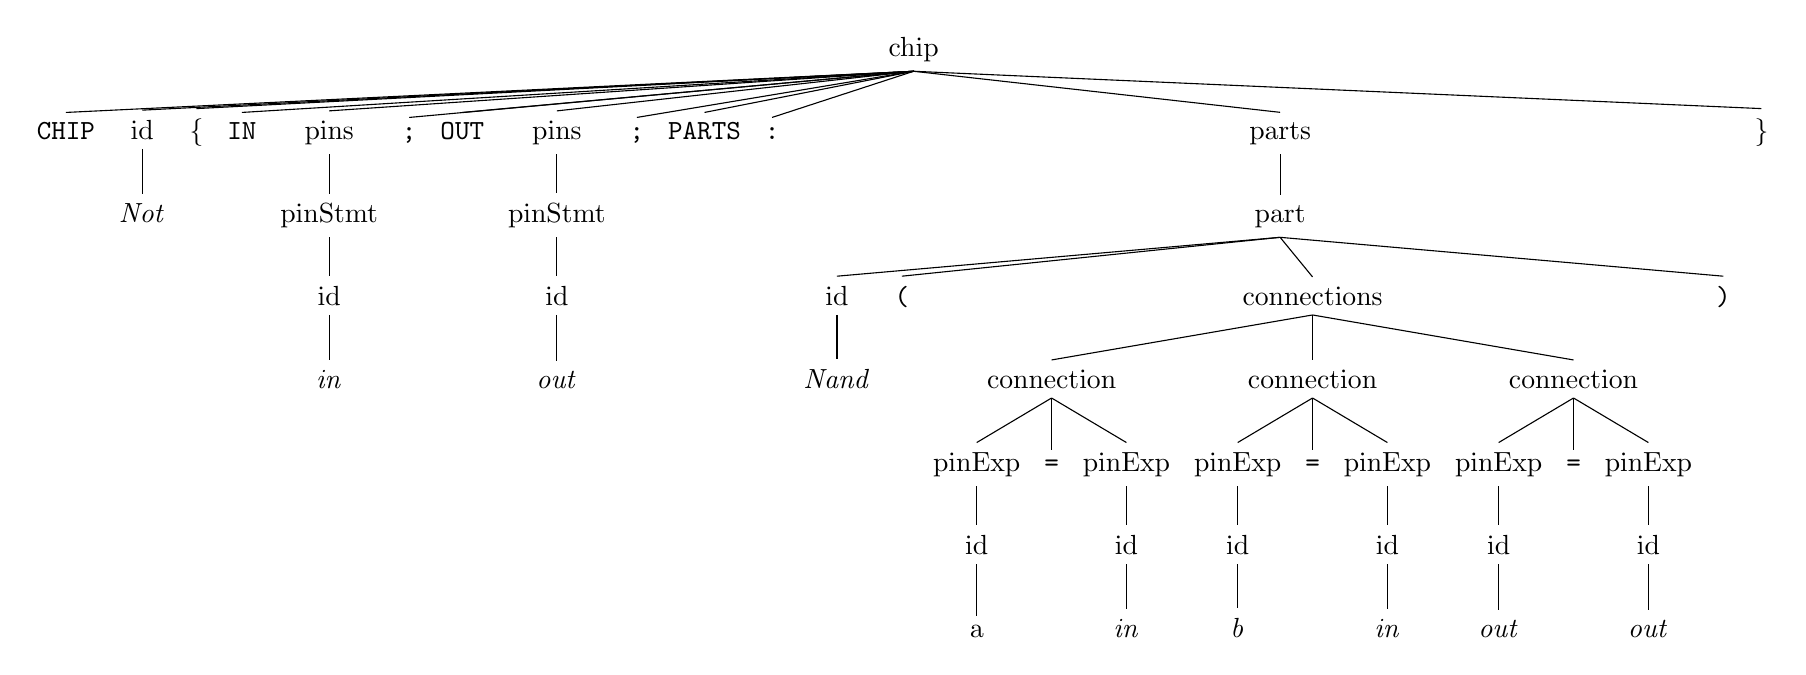
\begin{tikzpicture}
  \Tree [.chip
    [.\texttt{CHIP} ]
    [.id
      [.\textit{Not} ]
    ]
    [.\texttt{\{} ]
    [.\texttt{IN} ]
    [.pins
      [.pinStmt
        [.id
          [.\textit{in} ]
        ]
      ]
    ]
    [.\texttt{;} ]
    [.\texttt{OUT} ]
    [.pins
      [.pinStmt
        [.id
          [.\textit{out} ]
        ]
      ]
    ]
    [.\texttt{;} ]
    [.\texttt{PARTS} ]
    [.\texttt{:} ]
    [.parts
      [.part
        [.id
          [.\textit{Nand} ]
        ]
        [.\texttt{(} ]
        [.connections
          [.connection
            [.pinExp
              [.id
                [.a ]
              ]
            ]
            [.\texttt{=} ]
            [.pinExp
              [.id
                [.\textit{in} ]
              ]
            ]
          ]
          [.connection
            [.pinExp
              [.id
                [.\textit{b} ]
              ]
            ]
            [.\texttt{=} ]
            [.pinExp
              [.id
                [.\textit{in} ]
              ]
            ]
          ]
          [.connection
            [.pinExp
              [.id
                [.\textit{out} ]
              ]
            ]
            [.\texttt{=} ]
            [.pinExp
              [.id
                [.\textit{out} ]
              ]
            ]
          ]
        ]
        [.\texttt{)} ]
      ]
    ]
    [.\texttt{\}} ]
  ]
\end{tikzpicture}
\end{document}
